\subsection{Ajout de compétences}
\label{S ajout de competences}
Afin d'essayer d'augmenter la complexité du problème et de le rapprocher du réel, nous introduisons ici la compétence des techniciens. Nous disposons de 2 compétences A \& B et nous attribuons les compétences aux techniciens de manière suivante :
\begin{itemize}
    \item $\lfloor$20\%$\rfloor$ des techniciens sont des 2 compétences A et B
    \item $\lfloor$40\%$\rfloor$ de compétence A
    \item $\lfloor$40\%$\rfloor$ de compétence B
    \item le reste n'a pas de compétence spécifique
\end{itemize}
\\

Les clients ont aussi des demandes spécifiques aux différents services. Voici la répartition des clients:
\begin{itemize}
    \item 15\% des deux services A \& B
    \item 30\% du service A
    \item 30\% du service B
    \item 15\% pas de service
\end{itemize}
\\

Des relations existent entre les différentes compétences. En effet, un client ayant besoin les deux services ne peut être satisfait que par un techniciens ayant les deux services. De plus, un client ayant besoin du service A (respectivement B) doit être servi par un technicien ayant le service A (respectivement B) ou les deux services A \& B. Les clients n'ayant pas besoin de compétence peuvent être servi par n'importe quel technicien.

Nous pénalisons dans la fonction objectif le fait qu'un client soit servi par un mauvais technicien par un terme qui est 3 fois la distance entre le dépôt et ce client. Par exemple, un client A servi par un technicien B ou un client A \& B servi par un technicien B.\\


Nous avons modifié la structure de données pour qu'elle prenne en compte ces compétences. Pour cela, comme dans la partie \ref{sub probleme du sacados}, nous trions les clients en ordre décroissant de la demande. En suite, nous mettons les clients de type A \& B dans les tournées A \& B, si le nombre de tournées de ce type n'est pas suffisant, nous mettons le reste des clients A \& B de côté. La même procédure est appliquée pour les clients de type A (respectivement B) avec les tournées A (respectivement B). Enfin, tous les clients restant sont placés dans les tournées sans prendre en compte les compétences avec l'algorithme \textit{First Fit Decreasing}.

Les étapes suivantes de l'heuristique sont inchangées car elles évaluent les tournées avec la fonction objectif qui est déjà implémentée et qui prend en compte les pénalités des clients mal servi.
 \newpage
\begin{center}
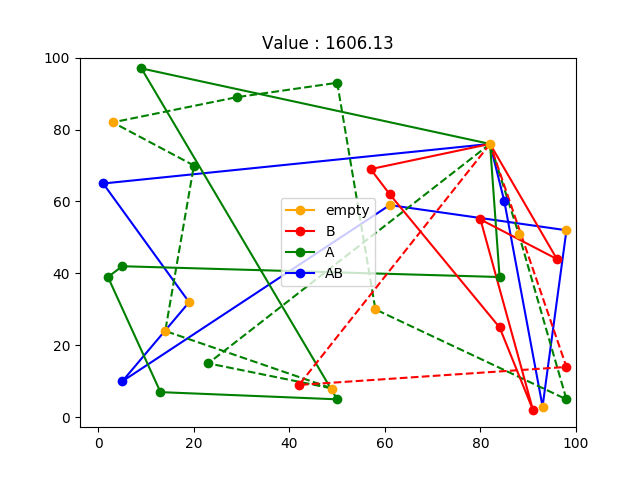
\includegraphics[width=0.49\linewidth]{pictures/image4.png}
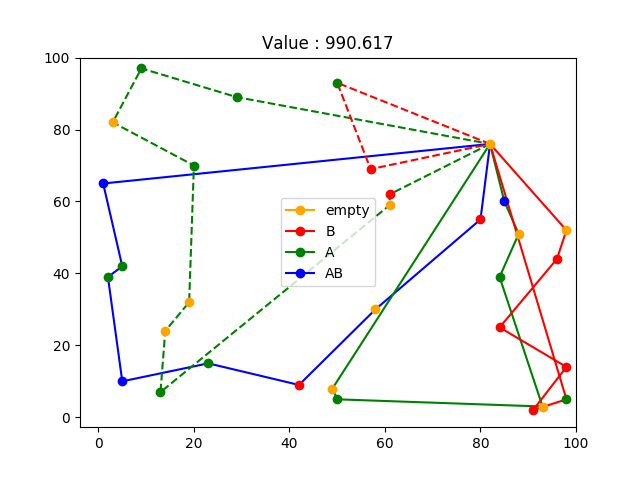
\includegraphics[width=0.49\linewidth]{pictures/image6.png}
\captionof{figure}{Tournées obtenues par heuristiques : a) Construction b) Recuit simulé pour \texttt{A-n32-k5}}
\end{center}

Nous observons dans la figure ci-dessus les solutions retournées à différentes étapes de l'heuristique. En a), nous pouvons voir la solution retournée par l'heuristique de construction, elle a une valeur de 1606. En b), nous avons la solution retournée par le recuit simulé avec une valeur de 990. Ce que nous pouvons remarquer dans cette figure c'est que la valeur de la solution est meilleur après l'application du recuit simulé. Nous constatons que les clients sont globalement attribués dans les service correspondant.
\\

Ensuite, nous avons modifié la PLNE pour qu'elle soit adaptée à ce problème. En ajoutant une troisième dimension k aux variables $x_{ij}$. Nous fixons le nombre de tournées à m. Une autre variable, $p^k_{0j}$, est ajoutée dans la fonction objectif, elle est décrite de la manière suivante :
\[
p^k_{0j} =
\begin{cases}
\text{distance entre le dépôt et le client j s'il est servi dans la mauvaise tournée k}\\
0 \text{ sinon}
\end{cases}
\]
\newpage

La PLNE devient :
\[\text{Min} \sum_{(i, j) \in A} (c^k_{ij} + 3p^k_{0j})x^k_{ij}\]

\[\begin{cases}
{\mathlarger\sum_{j=1}^{n}} x^k_{0j} = 1, \forall k \in \{0, ..., m\} \\
{\mathlarger\sum_{i=1}^{n}} x^k_{i0} = 1, \forall k \in \{0, ..., m\} \\
{\mathlarger\sum_{k=0}^{m}} x^k_{0j} \leq 1, \forall j \in \{0, ..., n\}\\
{\mathlarger\sum_{k=0}^{m}} x^k_{i0} \leq 1, \forall i \in \{0, ..., n\}\\
{\mathlarger\sum_{j=0}^{n}} x^k_{ij} \leq 1, \forall i \in \{0, ..., n\}, \forall k \in \{0, ..., m\}\\
{\mathlarger\sum_{i=0}^{n}} x^k_{ij} \leq 1, \forall j \in \{0, ..., n\}, \forall k \in \{0, ..., m\}\\
{\mathlarger\sum_{k=0}^{m}}{\mathlarger\sum_{j=0}^{n}} x^k_{ij} = 1, \forall i \in \{0, ..., n\}\\
{\mathlarger\sum_{k=0}^{m}}{\mathlarger\sum_{i=0}^{n}} x^k_{ij} = 1, \forall j \in \{0, ..., n\}\\
x^k_{ij} \in \{0,1\}, \forall (i, j) \in A, \forall k \in \{0, ..., m\}
\end{cases}\]

Ces contraintes modélisent l'ensemble du problème mais elles ne sont pas suffisantes pour avoir plus d'information sur chaque tournée. Les valeurs retournées dans la fonction \textit{callback} ne nous permettent pas de couper les points.

Avec cet aspect, le problème devient plus facile pour les heuristiques. En effet, le problème est moins "combinatoire" parce que le seul moyen de résoudre ce problème est de placer au mieux les clients dans les tournées correspondantes à leur besoin.